
\chapter{Test Converter}
Figure \ref{fig:Phase3_Architecture} represents architecture that proposes implementing Test Converter as a separate module. The main idea driving us was having a clean architecture that would make the Test Driver easily maintainable and extensible. Thus, we will separate these two even more and implement them as two different Java console applications. Test Driver will only handle executing the test-cases on Rumble. Test Converter will only handle converting the XQuery test suite to a JSONiq one, basically, it covers orange blocks from Figure \ref{fig:Phase3_Architecture}. 

However, In Section \ref{Phase3_Description}, we have explained the downsides of hard-coded conversion using Java String.replace method. Just having the clean architecture would not solve the hard-coding issues in Test Converter. Ultimately, we want to produce purely JSONiq Test Suite (similar to QT3TS for XQuery). Such Test Suite would be available for everyone to use and verify other JSONiq implementations such as Zorba \cite{Zorba}, IBM WebSphere \cite{WebSphere}, Xidel \cite{Xidel}.

\section{Rumble Architecture}
First, we need to think about achieving a clean XQuery to JSONiq conversion without hard-coding. Let us recall Rumble and its entire Section \ref{sec:RumbleArchitecture}. We said that in order to finally execute the query, we are performing conversion from Expression Tree to a tree of runtime iterators. The Expression Tree itself is a higher-level abstraction of JSONiq functional language that is composed of expressions. The entire Node class hierarchy that was implemented in Rumble is used to represent the Expression Tree.

If we can create an Expression Tree from a query written in XQuery, it would mean that we have created JSONiq Expression Tree. Instead of creating the runtime iterator and executing the query, we can just serialize Expression Tree to JSONiq query directly. We will reuse Rumble and extend its architecture so that it supports parsing queries written in XQuery. 

This means that even though Test Converter and Test Driver will be two separate Java console applications, they will both use Rumble. One may argue that the success of standalone JSONiq Test Suite will in that case depend on Rumble implementation. And this is true, it will. Nevertheless, the decision here is to use Rumble simply because using JSONiq Expression tree Rumble is the cleanest possible solution for conversion. Finally, it will also improve Rumble itself by supporting an additional query language - XQuery.

In Figure \ref{fig:Rumble_General_Architecture_With_XQuery} we have represented that will enable us to achieve the target. In the following sub-sections, we will explain XQuery Lexer \& Parser and Translator's implementation details together with the Serialization part. 

\begin{figure}[h!]
	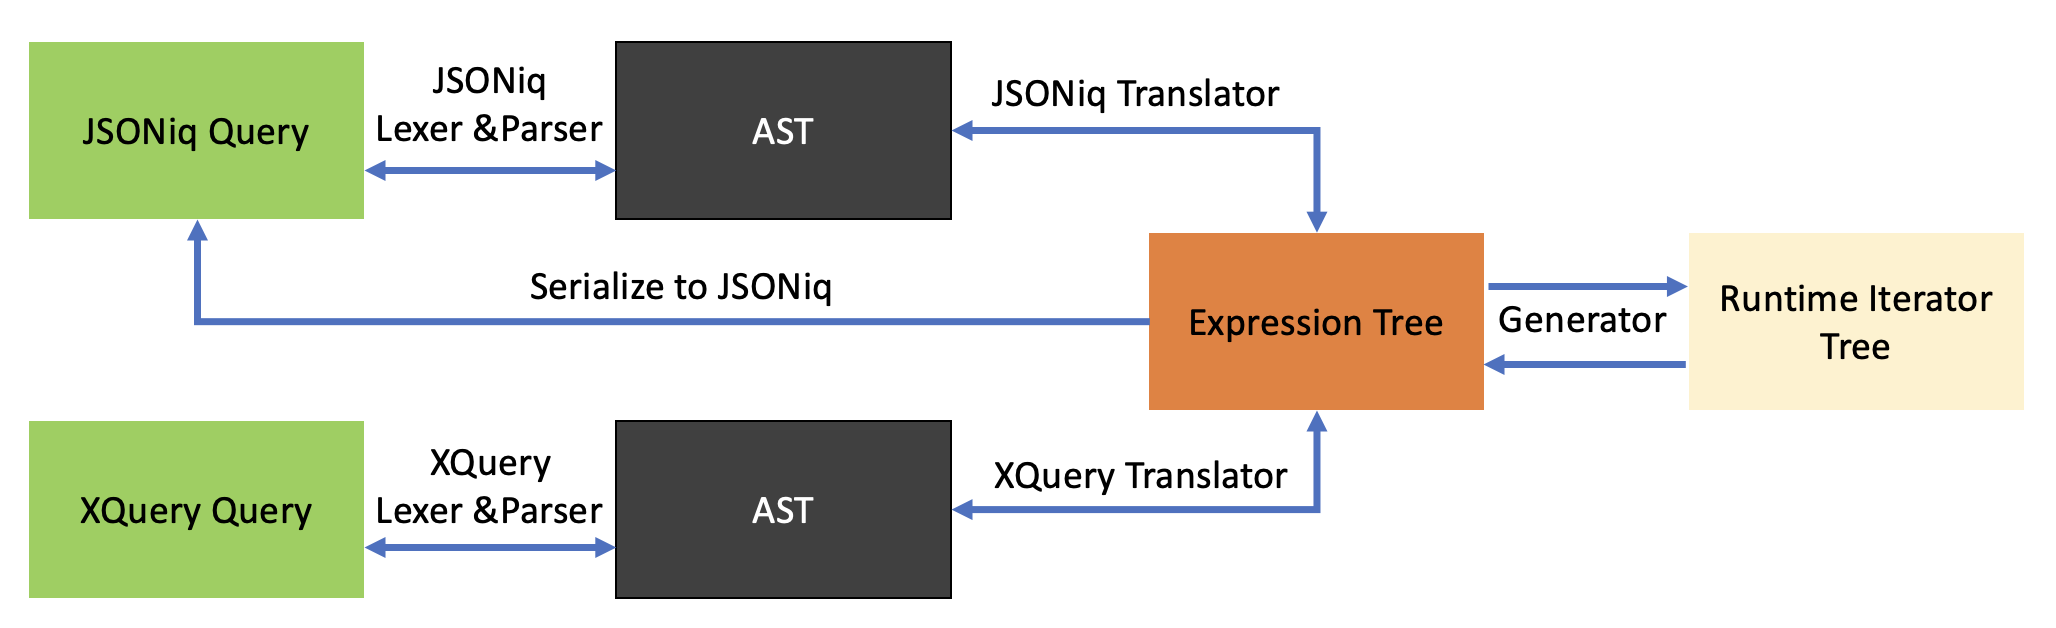
\includegraphics[width=\linewidth]{double_parsing_architecture.png}
	\vspace*{-5mm}
	\caption{Rumble General Architecture with XQuery}
	\label{fig:Rumble_General_Architecture_With_XQuery}
\end{figure}

\section{Rumble Extension}
Here we will go into details of the implementation of each and every modification that has been performed in Rumble in order for us to be able to reuse the already existing classes in the Node class hierarchy. 

\subsection{Lexer and Parser}
If we recall Section \ref{sec:RumbleLexerParser}, for simple languages, these two modules can be automatically generated from the grammar of the language. XQuery is 95\% similar to JSONiq. Thus, we need to create a grammar file similar to JSONiq.g4. 

The initial approach was to implement the XQuery.g4 file ourselves based on the already implemented JSONiq.g4 file in Rumble. However, XQuery is older than JSONiq and it was logical that such a file was already implemented. Indeed, we managed to find an ANTLR4 implementation of xqDoc for XQuery \cite{XqueryGrammar}. It is licensed under the same Apache License 2.0 as Rumble, and we can reuse it. The grammar is stable and it was not changed for more than 10 months, so we do not expect it to be updated. Also it is compliant with XQuery 3.1 W3C Recommendation \cite{XQueryRecommendation}. 

Names of certain labels in the grammar file were changed in order to match the code of TranslationVisitor class, which will be used as a baseline to implement XQueryTranslationVisitor. The structure remains the same except for:
\begin{enumerate}
	
	\item module was not according to the W3C Recommendation \cite{XQueryRecommendation} and allowed for multiple mainModules. See below the comparison between old and new module implementation.
	
	module : xqDocComment? versionDecl? xqDocComment? (libraryModule $|$ (mainModule (SEMICOLON versionDecl? mainModule)*));
	
	module : xqDocComment? versionDecl? xqDocComment? (libraryModule $|$ mainModule) ;
	\item moduleDecl was changed to use uriLiteral instead of stringLiteral in order to match the implementation of TranslationVisitor class. This does not affect the structure as uriLiteral comes down to stringLiteral in the next level of nesting (uriLiteral: stringLiteral)
	\item prolog was changed to use annotatedDecl in order to match the implementation of TranslationVisitor class. This does not affect the structure as annotatedDecl offers the same options that were originally in prolog:
	
	annotatedDecl: varDecl $|$ functionDecl	$|$ contextItemDecl $|$ optionDecl;
	
	\item functionDecl and varDecl were not according to the W3C Recommendation \cite{XQueryRecommendation}. It allowed for (annotations $|$ ncName) while the ncName is under annotations but on 3 levels below in nesting
 	
	\item varDecl was not according to the W3C Recommendation \cite{XQueryRecommendation}. varValue and varDefaultValue were defined as expr instead of exprSingle and it allowed them to be surrounded by \{ \}. See below the comparison between old and new varDecl implementation.
	
	varDecl: KW\_DECLARE annotations KW\_VARIABLE DOLLAR varName typeDeclaration?
	(
	(COLON\_EQ varValue)
	$|$ (KW\_EXTERNAL (COLON\_EQ varDefaultValue)?)
	$|$ (LBRACE varValue RBRACE)
	$|$ (KW\_EXTERNAL(LBRACE varDefaultValue RBRACE)?)
	) ; 
	
	varDecl: KW\_DECLARE annotations KW\_VARIABLE DOLLAR varName typeDeclaration?
	((COLON\_EQ varValue)
	$|$ (KW\_EXTERNAL (COLON\_EQ varDefaultValue)?)) ;
	
	varValue: expr ; $->$ varValue: exprSingle ;
	
	varDefaultValue: expr ; $->$ varDefaultValue: exprSingle ;
	
	\item squareArrayConstructor was changed to use expr instead of exprSingle (COMMA exprSingle)* in order to match the implementation of TranslationVisitor class. This does not affect the structure as it is equivalent in the next level of nesting (expr: exprSingle (COMMA exprSingle)* ;)
	
	\item arrowExpr was changed to use complexArrow instead of arrowFunctionSpecifier argumentList in order to match the implementation of TranslationVisitor class. This does not affect structure as it is equivalent in next level of nesting (complexArrow: arrowFunctionSpecifier argumentList;)
\end{enumerate}

We have also implemented another script for handling the XQuery.g4, and using it, ANTLR auto-generated XQueryParser and XQueryLexer together with its corresponding XQueryParserBaseVisitor base class.

\subsection{Translator}
The second part requires us to implement XQueryTranslationVisitor that extends the generated XQueryParserBaseVisitor class and wraps around the Node class. With proper implementation, we would be able to achieve converting XQuery into the JSONiq Expression Tree. The implementation is mainly based on the already implemented JSONiq TranslationVisitor with modifications that we will document here.

Of course, not everything can be converted to JSONiq and it should not be converted. Below we will list the conversions that we have left out as they will never be supported:
\begin{itemize}
	\item schemaImport
	\item copyNamespacesDecl
	\item constructionDecl
	\item boundarySpaceDecl
	\item optionDecl
	\item nodeComp
	\item unionExpr
	\item intersectExceptExpr
	\item parenthesizedExpr within the arrowFunctionSpecifier of arrowExpr
	\item URIQualifiedName
	\item validateExpr, extensionExpr within valueExpr of unaryExpr
	\item nodeConstructor within primaryExpr
	\item kindTest, typedMapTest, typedArrayTest within itemType
	\item axisStep within stepExpr
	\item multiple stepExpr within relativePathExpr
	\item single or double dash preceding relativePathExpr within pathExpr
\end{itemize}

In addition to that, there are conversions that we are yet not able to perform as the implementation is missing in Rumble. As Rumble implementation improves, so will the implementation of XQueryTranslationVisitor as well. For now, following conversions are classified as out of scope of the thesis and will be supported in future once Rumble is upgraded:
\begin{itemize}
	\item defaultNamespaceDecl
	\item decimalFormatDecl
	\item baseURIDecl
	\item contextItemDecl
	\item existUpdateExpr within exprSingle
	\item parenthesizedExpr and STAR object lookup within keySpecifier of lookup
	\item orderedExpr and unorderedExpr within primaryExpr
	\item windowClause within initialClause of flworExpr
	\item functionTest within itemType
\end{itemize}

For the versions that we support, since the grammar file is based on the XQuery 3.1 W3C Recommendation \cite{XQueryRecommendation}, we have decided to support XQuery versions 1.0, 3.0 and 3.1 as version  3.1 is backward compatible.

For annotations, currently, we only support single public annotations without prefix. Single since we can see from QT3TS in the prod/ModuleImport.xml, tests modules-pub-priv-29 to 36, we can see that "It is an error if a variable's annotations contains any combination of two annotations". In addition, according to the W3C Recommendation \cite{XQueryRecommendation} it is said that "If no prefix is present, the name is in the "http://www.w3.org/2012/xquery namespace". This results in following implementation of annotation handling:
\begin{enumerate}
	\item Throw an error if there is more than 1 annotation in the annotations list
	\item Otherwise, extract the EQName
	\item Throw an error if prefix is not equal to http://www.w3.org/2012/xquery 
	\item Otherwise, throw an error if local name is not public
	\item Otherwise, let the query with annotations be converted
\end{enumerate}

Namespaces fn and map that were removed in Section \ref{Phase2_Converter}, we are now binding. Namespace xs is part of grammar. For namespaces map and array, no binding is needed as they are counted for Item 2 as mentioned in Section \ref{sec:TestConverterImplementation}

Handling the Literals is slightly different. If we compare JSONiq with XQuery, we will see that true, false and null literals do not exist in XQuery. Instead, they will be added as function calls.

The itemType of XQuery covers more possibilities compared to the JSONiq:

itemType: kindTest
$|$ (KW\_ITEM LPAREN RPAREN)
$|$ functionTest
$|$ mapTest
$|$ arrayTest
$|$ atomicOrUnionType
$|$ parenthesizedItemTest ;

itemType                : Kitem
$|$ atomicType;
$|$ Kobject
$|$ Karray
$|$ Kjson;

In JSONiq TranslationVisitor implementation, it was enough to call getItemTypeByName method and pass the parsed context. In XQuery implementation, this is only possible for the atomicOrUnionType. For all others, we have to handle it differently. First of all, kindTest will throw an error as it corresponds to the 7 complex (non-atomic) types that should not be converted (document, element etc.). FunctionTest is not yet supported in Rumble and it is out of the scope of the thesis. The mapTest and arrayTest correspond to AtomicItemType.Object and AtomicItemType.Array item type of JSON if they are untyped, otherwise we throw an error. Item is the AtomicItemType.item while parenthesizedItemTest recursively calls the same method.

When it comes to arrayConstructor, there is a slight problem. JSONiq and XQuery do not have the same data model - there is a data model mismatch. XQuery allows us to have a Sequence of Items as array members or object values. JSONiq does not support that and requires single items instead. The only way to store a Sequence of Items in the JSONiq data model is using arrays. In order to overcome the dependency mismatch, we introduce mapping between two data models and we map nested Sequence of Items of XQuery to JSONiq array. In the case of squareArrayConstructor of XQuery, we recursively iterate over the exprSingle in expression and perform visitExprSingle. Each expression returned by visitExprSingle, is then wrapped into an array constructor. Finally, all these array constructors are wrapped into Comma Expression that is then wrapped in the main array constructor. In the case of curlyArrayConstructor, we first obtain the content by calling visitExpr. Then we instantiate a new Context Item Expression and wrap it into an array constructor. We combine these two by instantiating a new Simple Map Expression and wrap it in the main array constructor.

\subsection{Serialize to JSONiq}
Instead of running the query and returning the iterator over the resulting Sequence of Items, we need to perform serialization. Serialization is basically an inverted process of parsing. We have declared a new method serializeToJSONiq in the abstract class Node. All other classes used to create the JSONiq Expression Tree are derived from Node, and in those classes, we need to implement the method. We are now peeking into the XQuery.g4 grammar file in order to recreate the String representation of each and every Expression. In each implementation, we use the appropriate keywords and recursively call serializeToJSONiq for each nested Expression. 

In Section \ref{sec:RumbleArchitecture}, we have presented the 4 phases that Rumble goes through as a compiler. If we further analyze these phases through the code of Java Rumble API, we can identify the following steps that are required in order to execute the query:
\begin{enumerate}
	\item Instantiate Lexer from the input stream - this is the complete query
	\item Instantiate Parser using the Lexer from Step 1
	\item Instantiate Static Context  (map between variable names and sequence types) using the URI file - this is the input file on which the query is executed 
	\item Instantiate Translation Visitor using Static Context from Step 3
	\item Instantiate MainModule by calling visit method of Translation Visitor and passing the main module extracted by the Parser as the argument
	\item In the runQuery method of Java Rumble API, first 5 Steps are performed by calling parseMainModuleFromQuery method that returns Main Module from Step 5
	\item Instantiate Dynamic Context (mapping between variable names and actual sequences of items) using returned Main Module from Step 6
	\item Instantiate RunTimeIterator using returned Main Module from Step 6
	\item Return the Sequence of Items result instantiated using the Iterator from Step 8 and Dynamic Context from Step 7
\end{enumerate}

To perform only serialization without obtaining the query results, we have extended Java Rumble API with an additional method serializeToJSONiq. This method performs the first same first 6 Steps described above. After that, we simply call the implementation of serializeToJSONiq of abstract Node class via Main Module from Step 6. We pass String Buffer as the argument, which gets populated and then the Java Rumble API serializeToJSONiq method returns it as a String. Such implementation allowed Rumble to provide conversion out of the box via JSONiq Expression Tree.

\section{Architecture}
\label{sec:TestConverterImplementation}
As we said before in Section \ref{Phase3_Description} we will distinguish 6 cases, but for this implementation we will need only first 2: 
\begin{enumerate}
	\item Fails, as expected and should not be converted to JSONiq. It will never be supported. - Documented in Table \ref{tab:Phase3_Item1}
	\item Fails, as expected since it is not supported yet - Documented in Table \ref{tab:Phase3_Item2}
	\todo{@Ghislain Fourny - These two were also compiled during our email exchange in the Excel sheet. Do I need to cite anything?}
\end{enumerate}

This separation is important to understand. As we want to produce a standalone JSONiq Test Suite similar to QT3TS for XQuery, all Item 1 should not be included as they are not JSONiq. On the other hand, all Item 2 should be included because they can be used to verify other JSONiq implementations. 

The final architecture of the Test Converter can be seen in Figure \ref{fig:test_converter_final_architecture.png}. There is a slight difference compared to Test Driver architecture. Test Converter does not need to execute the JSONiq query. Therefore as presented in Figure \ref{fig:Rumble_General_Architecture_With_XQuery}, we will simply call serializeToJSONiq instead of creating runtime iterators that would be executed on top of Spark, i.e. we do not need Spark. 

\begin{figure}[h!]
	\vspace*{-5mm}
	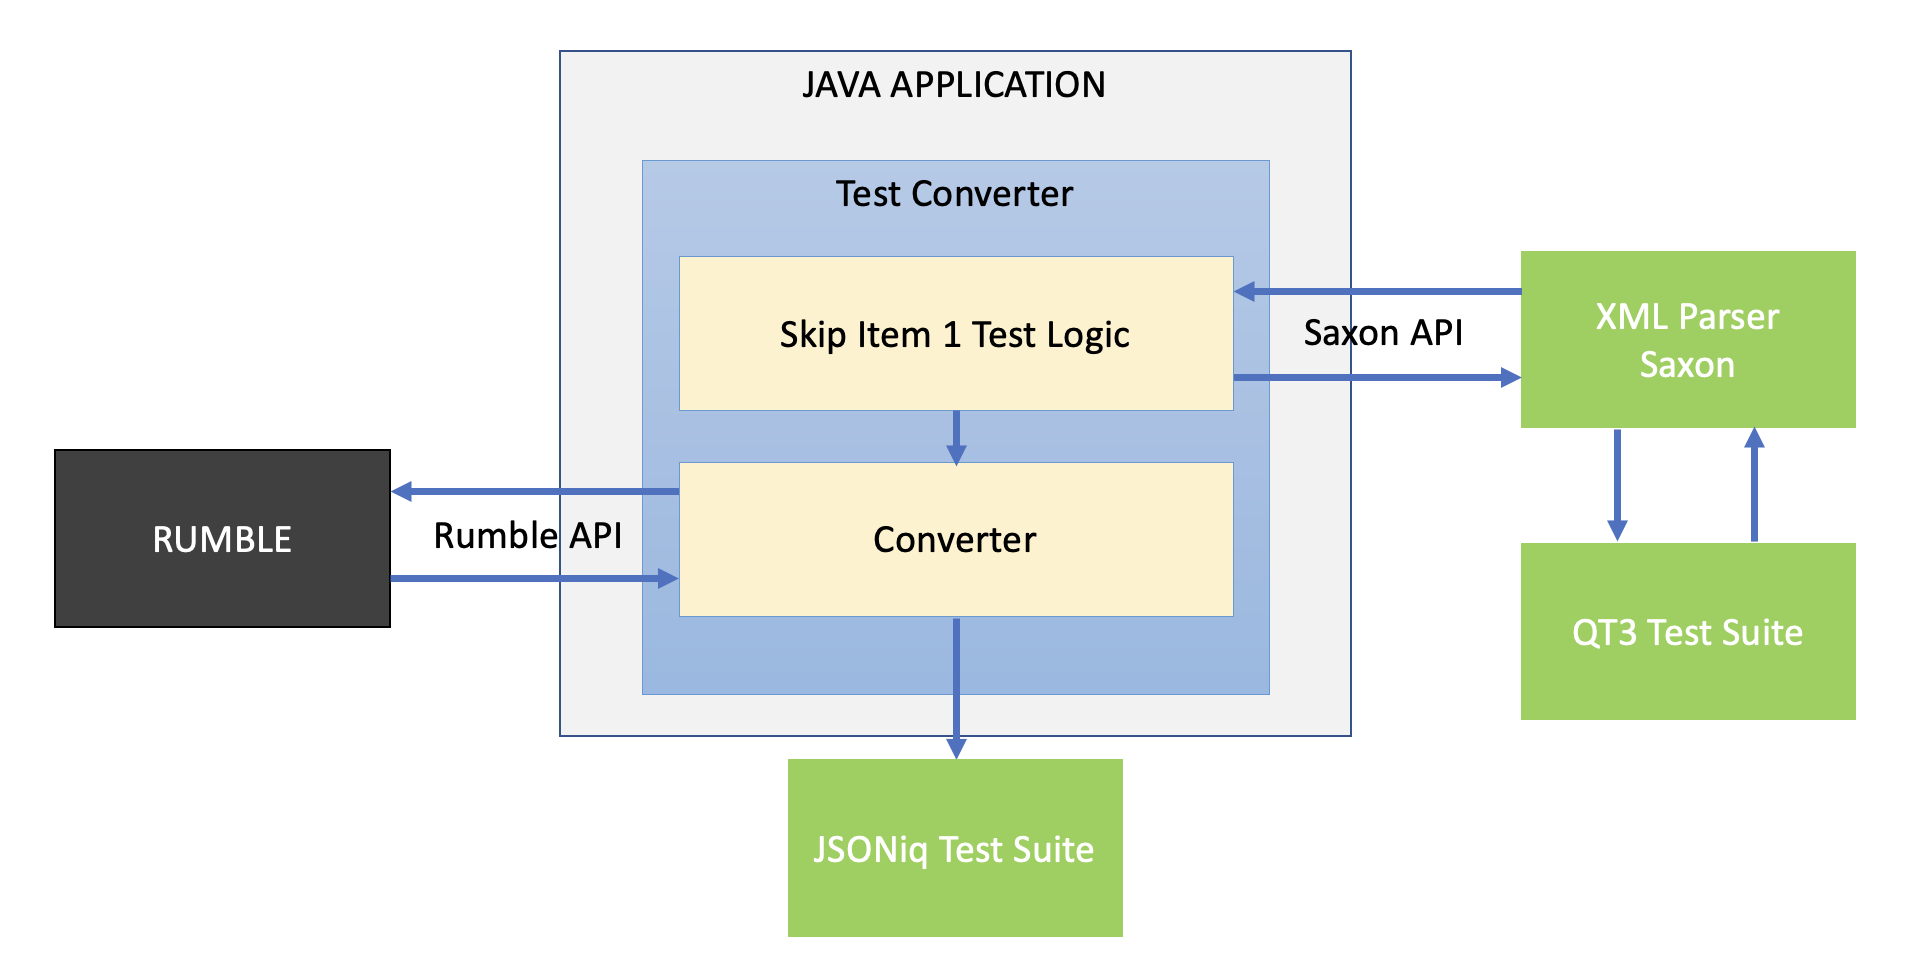
\includegraphics[width=\linewidth]{test_converter_final_architecture.png}
	\vspace*{-8mm}
	\caption{Test Converter Final Architecture}
	\label{fig:test_converter_final_architecture.png}
\end{figure}

\vspace*{-4mm}
Final Test Driver architecture can be seen in Figure \ref{fig:test_driver_final_architecture.png}. We will maintain a list of Item 2 that will not be executed in Test Driver for Rumble. Test Driver will now take JSONiq Test Suite produced by Test Converter and execute it. 

\begin{figure}[h!]
	\vspace*{-5mm}
	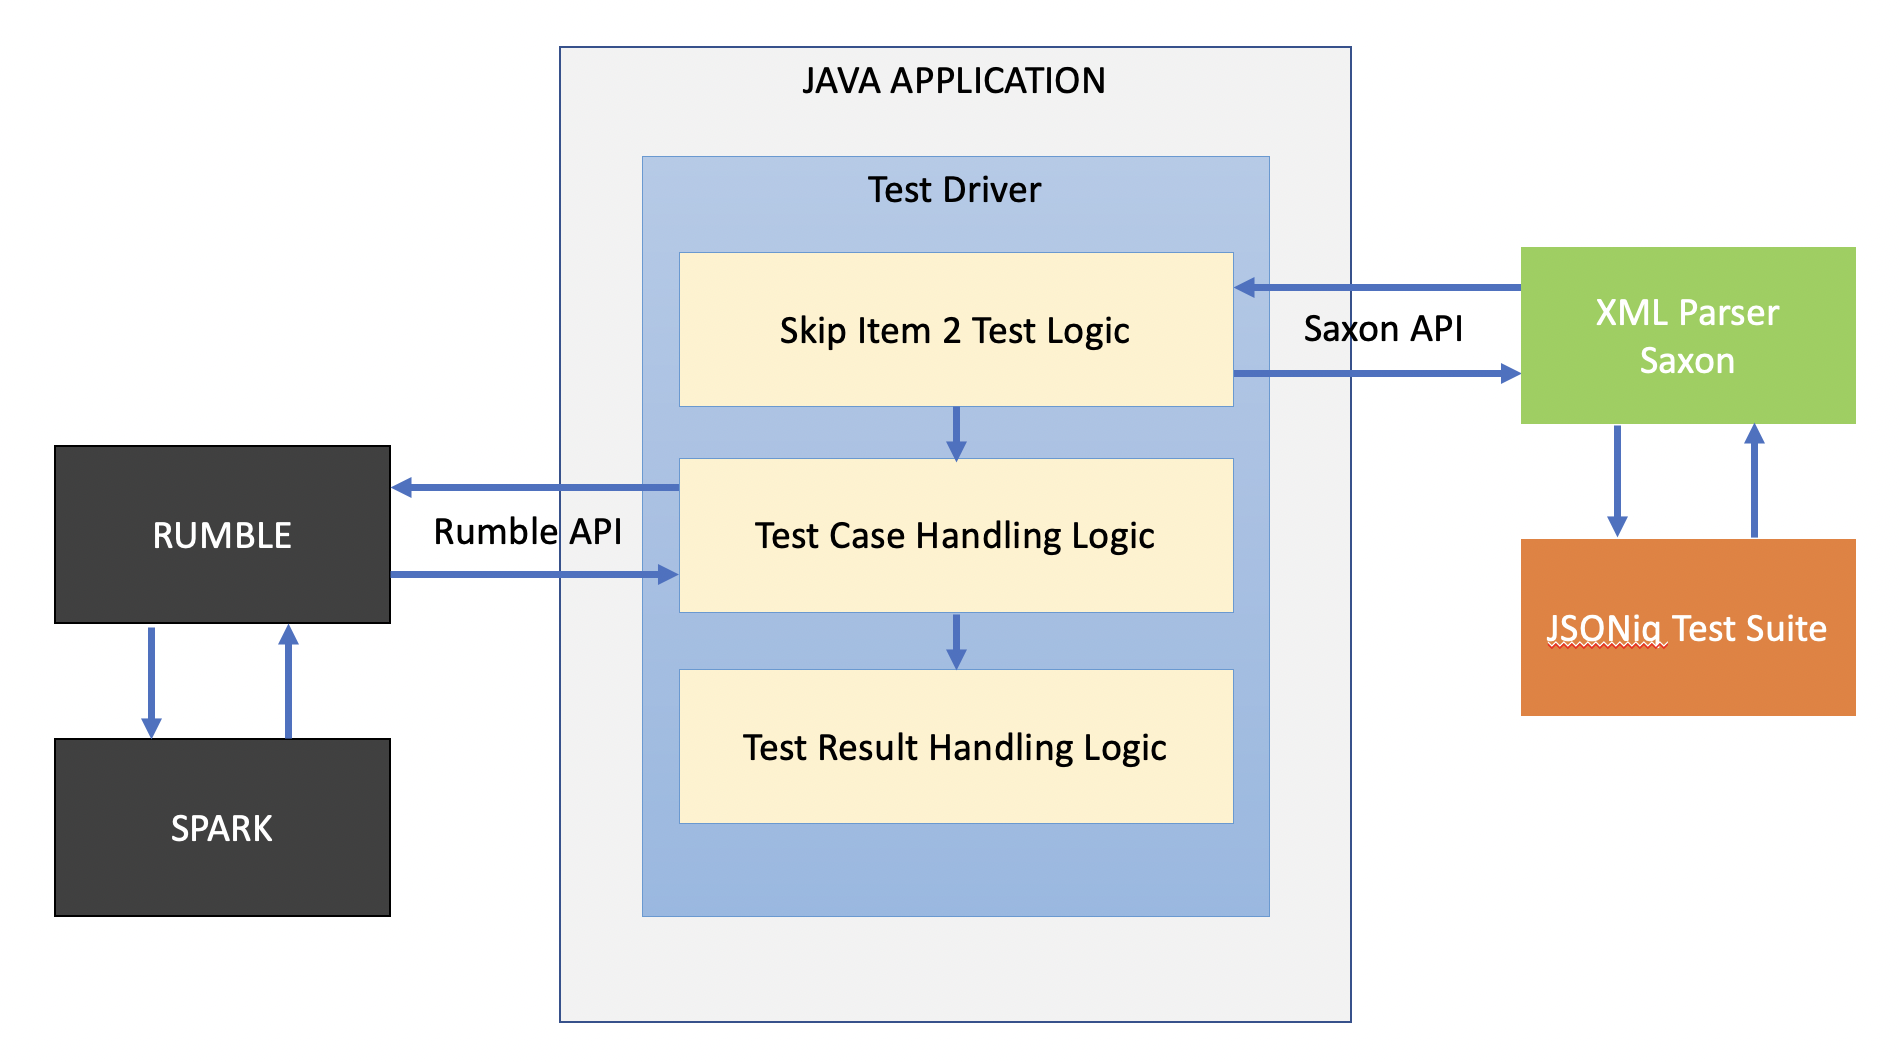
\includegraphics[width=\linewidth]{test_driver_final_architecture.png}
	\vspace*{-8mm}
	\caption{Test Converter Final Architecture}
	\label{fig:test_driver_final_architecture.png}
\end{figure}

\section{Implementation}
The Converter part is using method binding provided by Saxon. First, we define the ExtensionFunction and the name under which it will be available in XQuery expression (convert). Secondly, we specify what the result of this function is (the result of the Java Convert method). Finally, we assign it a namespace (bf). We now declare XQuery expression that has a function that recursively visits all nested XML tags. In case that they are test or result tags, it will pass the under-laying tag value to bf:convert and replace the tag value with the returned result. We declare external variable and pass the entire test-set to the XQuery expression. Check the code below:

\lstinputlisting[language=Java, frame=single, breaklines=true, showspaces=false, stringstyle=\color{ao}, keywordstyle=\color{chromeyellow}, basicstyle=\tiny]{source_code_method_binding.java}

The Java Convert method simply uses Rumble API to call serializeToJSONiq method we have previously created, making the conversion complete. There is a small remark to take into consideration here. The test-cases that have error codes will cause a RumbleException. Due to time constraints, we could not make a better classification and check for which error codes we need to perform XQuery to JSONiq conversion of test tag. Thus, those test-cases will not be converted and return the same result instead. Check the code below:

\lstinputlisting[language=Java, frame=single, breaklines=true, showspaces=false, stringstyle=\color{ao}, keywordstyle=\color{chromeyellow}, basicstyle=\small]{source_code_serializetojsoniq.java}

At the moment, Test Converter is dependent on Rumble as it was used to perform clean XQuery to JSONiq transformation. However, once Rumble is mature implementation supporting everything we have documented as missing, we will have a once and for all generated JSONiq Test Suite as our work output. 

On the other hand, Test Driver will not change much. We have a similar architecture as we had with the hard-coded conversion before but in a much cleaner approach. Test Driver can be used directly with either JSONiq or XQuery Test Suite depending on configuration, which we will explain in Section \ref{sec:overallsummary}. It will be helpful in improving the Rumble implementation by fixing and enable opening/closing issues and tracking the development progress of Rumble. Fixing the bugs and adding features will also consequentially lead to Item 2 list dropping down to 0. 
